% Final Viva Guide — personal study document, NOT a graded deliverable.
% Compile: xelatex Final_Viva_Guide.tex   (run twice for the table of contents)
\documentclass[11pt]{report}

\usepackage[margin=1in]{geometry}
\usepackage{amsmath}
\usepackage{amssymb}
\usepackage{fontspec}
\usepackage{graphicx}
\usepackage{booktabs}
\usepackage{longtable}
\usepackage{array}
\usepackage{xcolor}
\usepackage{caption}
\usepackage{enumitem}
\usepackage{tikz}
\usetikzlibrary{arrows.meta,positioning,shapes.geometric,fit,backgrounds,calc,matrix}
\usepackage{pgfplots}
\pgfplotsset{compat=1.18}
\usepackage[most]{tcolorbox}
\usepackage{listings}
\usepackage{titlesec}
\usepackage{fancyhdr}
\PassOptionsToPackage{hyphens}{url}
\usepackage[colorlinks=true,linkcolor=blue!50!black,urlcolor=blue!50!black,citecolor=blue!50!black]{hyperref}
\emergencystretch=3em
\sloppy

\newfontfamily\devanagarifont{Nirmala UI}
\newcommand{\dn}[1]{{\devanagarifont #1}}

\definecolor{hindiblue}{HTML}{1F6F8B}
\definecolor{nepalipurple}{HTML}{7A4FA3}
\definecolor{conceptgreen}{HTML}{2E8B57}
\definecolor{warnred}{HTML}{C0392B}
\definecolor{examplegold}{HTML}{B8860B}
\definecolor{codegray}{HTML}{F5F5F5}
\definecolor{titlenavy}{HTML}{102A43}

\titleformat{\chapter}[display]
  {\normalfont\huge\bfseries\color{titlenavy}}
  {\chaptertitlename\ \thechapter}{20pt}{\Huge}
\titleformat{\section}
  {\normalfont\Large\bfseries\color{titlenavy}}{\thesection}{1em}{}
\titleformat{\subsection}
  {\normalfont\large\bfseries\color{hindiblue}}{\thesubsection}{1em}{}

\pagestyle{fancy}
\fancyhf{}
\fancyhead[L]{\small\textit{Final Viva Guide}}
\fancyhead[R]{\small\leftmark}
\fancyfoot[C]{\thepage}
\renewcommand{\headrulewidth}{0.4pt}

\newtcolorbox{concept}[1]{colback=conceptgreen!6,colframe=conceptgreen,
  fonttitle=\bfseries,coltitle=white,colbacktitle=conceptgreen,
  title={\textbf{In simple words: #1}},sharp corners=south,boxrule=1pt,left=2mm,right=2mm,breakable}

\newtcolorbox{implementation}[1]{colback=hindiblue!6,colframe=hindiblue,
  fonttitle=\bfseries,coltitle=white,colbacktitle=hindiblue,
  title={\textbf{In my project: #1}},sharp corners=south,boxrule=1pt,left=2mm,right=2mm,breakable}

\newtcolorbox{example}[1]{colback=examplegold!8,colframe=examplegold,
  fonttitle=\bfseries,coltitle=white,colbacktitle=examplegold,
  title={\textbf{Example: #1}},sharp corners=south,boxrule=1pt,left=2mm,right=2mm,breakable}

\newtcolorbox{notebox}[1][Note]{colback=gray!8,colframe=gray!60!black,
  fonttitle=\bfseries,left=2mm,right=2mm,title={\textbf{#1}},breakable}

\newtcolorbox{warnbox}[1][Watch out]{colback=warnred!8,colframe=warnred,
  fonttitle=\bfseries,coltitle=white,colbacktitle=warnred,
  left=2mm,right=2mm,title={\textbf{#1}},breakable}

\newtcolorbox{qabox}[1]{colback=nepalipurple!5,colframe=nepalipurple,
  fonttitle=\bfseries,coltitle=white,colbacktitle=nepalipurple,
  title={\textbf{Q: #1}},sharp corners=south,boxrule=1pt,left=2mm,right=2mm,
  breakable}

\newtcolorbox{saybox}{colback=conceptgreen!8,colframe=conceptgreen!70!black,
  left=2mm,right=2mm,boxrule=0.8pt,breakable,
  title={\textbf{Say this out loud}},fonttitle=\bfseries,coltitle=white,
  colbacktitle=conceptgreen!70!black}

\lstset{
  backgroundcolor=\color{codegray},
  basicstyle=\ttfamily\small,
  breaklines=true,
  frame=single,
  rulecolor=\color{gray!50},
  showstringspaces=false,
  columns=fullflexible,
}

\newcommand{\p}[1]{\texttt{#1}}
\newcommand{\MH}{\textcolor{hindiblue}{\textbf{Model H}}}
\newcommand{\ML}{\textcolor{nepalipurple}{\textbf{Model L}}}

\title{\Huge\textbf{Final Viva Guide}\\[0.3cm]
\Large Everything in This Project, Explained in Simple Words\\[0.2cm]
\large Phases 1, 2 and 3 --- Model H (Hindi) and Model L (Nepali)}
\author{Swaraj Kumar \\ \small 2025202016 \\[0.2cm]
\small \textit{Personal study document --- not a graded deliverable}}
\date{\today}

\begin{document}
\maketitle

\begin{tcolorbox}[colback=gray!8,colframe=gray!50!black,title={\textbf{How to use this document}}]
This is a study guide I wrote for myself so I can explain every part of this
project confidently in the final viva. It is \textbf{not} a course deliverable
and does not affect grading.

Every number in here comes from a file this project actually produced. Nothing
is invented. Where something was \emph{not} done, or was done wrongly and then
fixed, this guide says so plainly --- because an examiner will find those places
anyway, and it is much better to walk in already knowing them.

\medskip
\textbf{The language is deliberately simple.} Where a technical term appears, it
is explained the first time in a green ``In simple words'' box.

\medskip
\textbf{If you only have one hour:} read Chapter~\ref{ch:cheat} (the cheat
sheet), then Chapter~\ref{ch:bank} (the question bank), then
Chapter~\ref{ch:mistakes} (mistakes to own). Everything else exists to make
those three make sense.
\end{tcolorbox}

\tableofcontents

% =======================================================================
\chapter{The Cheat Sheet}
\label{ch:cheat}

If you forget everything else, remember this chapter.

\section{What I built, in three sentences}

\begin{enumerate}[leftmargin=*]
\item I built \textbf{two completely separate} GPT-style language models from
      scratch in PyTorch --- one for \textbf{Hindi} (called \MH, the
      higher-resource language) and one for \textbf{Nepali} (called \ML, the
      lower-resource language). They share no data, no tokenizer, no vocabulary
      and no weights.
\item I collected and cleaned the corpus myself, trained a tokenizer for each
      language separately, wrote the whole Transformer using only basic PyTorch
      layers, pretrained both models for about 11 hours each on a Tesla T4 GPU,
      and evaluated them.
\item Then I generated my own synthetic reasoning dataset in each language,
      finetuned each model on its own language only, and measured whether that
      taught the model to reason. \textbf{It did not} --- and the most
      interesting part of my project is the evidence showing why.
\end{enumerate}

\section{The three findings I lead with}

\begin{enumerate}[leftmargin=*]
\item \textbf{Perplexity and bits-per-byte disagree.} Perplexity says Hindi is
      41\% better. Bits-per-byte says Nepali is slightly better. Both numbers
      are correct --- most of the gap is a \emph{tokenizer artifact}, not a real
      quality difference.
\item \textbf{Both models independently grew the same attention structure.}
      Different languages, different tokenizers, different random seeds --- and
      both produced a ``previous-token head'' at layer 3. Nobody designed that.
\item \textbf{Finetuning taught the output format, not the reasoning.} Exact
      match jumped from 0\% to 35\%, which looks like success. It is not: on a
      fair forced-choice test both models sit at or below the 41.67\% chance
      rate.
\end{enumerate}

\section{Numbers to memorise}

\begin{center}
\begin{tabular}{@{}lrr@{}}
\toprule
\textbf{Architecture (identical for both)} & \multicolumn{2}{c}{} \\
\midrule
Layers / heads / model dim / FFN dim & \multicolumn{2}{r}{6 / 8 / 512 / 2048} \\
Head dimension $d_k$ & \multicolumn{2}{r}{64} \\
Context length & \multicolumn{2}{r}{512} \\
Dropout & \multicolumn{2}{r}{0.1, at four places} \\
\midrule
 & \textbf{Model H} & \textbf{Model L} \\
\midrule
Total parameters & 23,273,472 & 24,297,472 \\
Non-embedding parameters & 18,915,328 & 18,915,328 \\
Vocabulary & 8,000 (Unigram) & 10,000 (BPE) \\
Corpus tokens & 505,852,028 & 635,204,333 \\
Train-split tokens & 485,956,678 & 521,426,359 \\
Bytes per token & 8.875 & 11.441 \\
Test perplexity & \textbf{27.41} & 46.68 \\
Test bits-per-byte & 0.5382 & \textbf{0.4846} \\
Greedy repetition rate & 0.598 & 0.577 \\
Best chrF++ (at $T=1.0$) & 16.29 & 18.05 \\
Reasoning exact match & \textbf{35.15\%} & 29.45\% \\
Reasoning forced choice & 36.35\% & 39.30\% \\
Forced-choice chance rate & 41.67\% & 41.67\% \\
\bottomrule
\end{tabular}
\end{center}

\section{The one thing I must never get wrong}

\begin{warnbox}[I did NOT implement RoPE]
My positional encoding options are \p{"learned"}, \p{"sinusoidal"} and
\p{"none"}. I shipped \textbf{learned absolute}.

If the examiner asks about RoPE, the correct answer is to explain what RoPE does
and why I chose differently. Claiming I built it would collapse the moment they
open \p{model/transformer.py}. See Section~\ref{sec:rope}.
\end{warnbox}

% =======================================================================
\chapter{What This Project Is, In Plain Words}

\section{The task}

A language model is a program that, given some text, predicts the next piece of
text. That is all it does. Everything else --- answering questions, writing
essays --- comes out of doing that one thing very well.

The assignment asked me to build two of these, for two Indian languages with
different amounts of available data, and then compare them fairly. The point is
not to win a competition. The point is to understand \emph{why} the two models
differ.

\begin{concept}{Higher-resource vs lower-resource language}
A ``higher-resource'' language has a lot of text freely available on the
internet --- Hindi has hundreds of millions of words easily reachable. A
``lower-resource'' language has much less --- Nepali has far fewer websites,
fewer digitised books, fewer newspapers online.

The interesting research question is: \emph{when you give both languages the
same model size and roughly the same number of tokens, what actually differs?}
\end{concept}

\section{Why two separate models and not one multilingual model}

This was a hard rule in the assignment, and there is a good scientific reason
for it. If I trained one model on both languages with one shared vocabulary,
then any difference I measured could be explained by the two languages sharing
or competing for capacity. By keeping them completely separate, and by giving
them \emph{exactly the same architecture}, every difference in the results must
come from the data or the tokenizer.

\begin{implementation}{Identical non-embedding parameters}
Both models have exactly \textbf{18,915,328} non-embedding parameters. Same
depth, same width, same number of heads, same feed-forward size. The only
difference in total parameter count comes from the vocabulary size, which
changes the embedding table.

This is what lets me say ``the difference is data and tokenizer, not capacity''
and have it actually be true.
\end{implementation}

\section{The shape of the whole pipeline}

\begin{center}
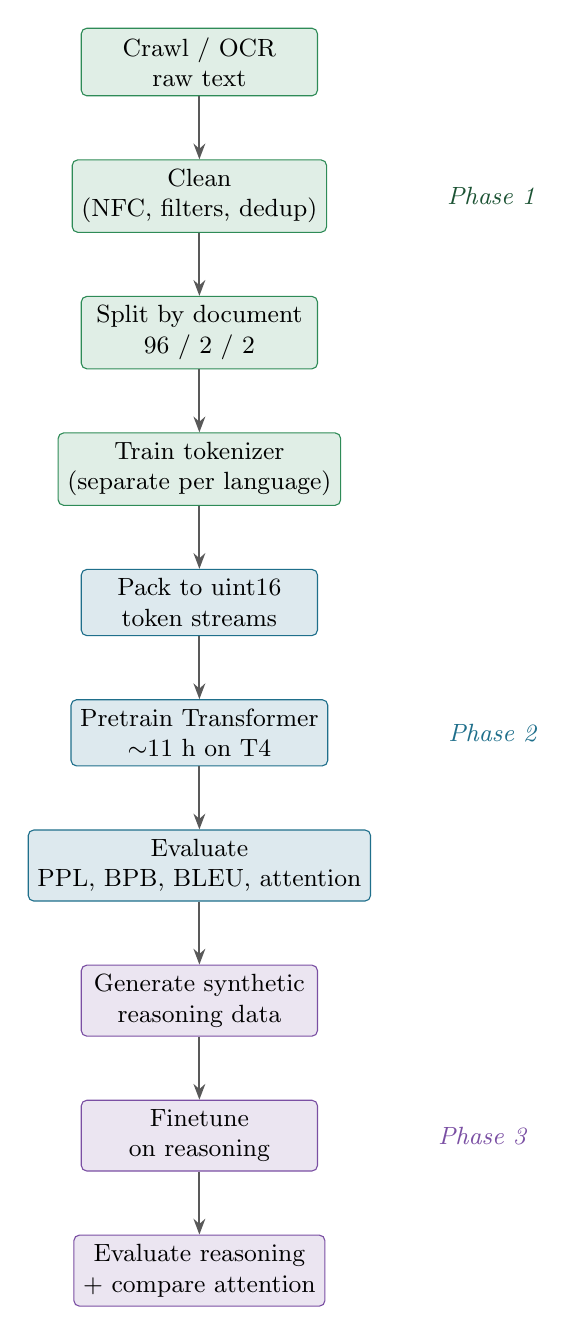
\begin{tikzpicture}[
  node distance=8mm,
  stage/.style={rectangle,draw,rounded corners=2pt,minimum width=30mm,
                minimum height=8mm,align=center,font=\small},
  p1/.style={stage,fill=conceptgreen!15,draw=conceptgreen},
  p2/.style={stage,fill=hindiblue!15,draw=hindiblue},
  p3/.style={stage,fill=nepalipurple!15,draw=nepalipurple},
  arrow/.style={-{Stealth[length=2mm]},thick,gray!70!black}
]
\node[p1] (raw) {Crawl / OCR\\raw text};
\node[p1,below=of raw] (clean) {Clean\\(NFC, filters, dedup)};
\node[p1,below=of clean] (split) {Split by document\\96 / 2 / 2};
\node[p1,below=of split] (tok) {Train tokenizer\\(separate per language)};
\node[p2,below=of tok] (pack) {Pack to uint16\\token streams};
\node[p2,below=of pack] (train) {Pretrain Transformer\\$\sim$11 h on T4};
\node[p2,below=of train] (eval) {Evaluate\\PPL, BPB, BLEU, attention};
\node[p3,below=of eval] (gen) {Generate synthetic\\reasoning data};
\node[p3,below=of gen] (ft) {Finetune\\on reasoning};
\node[p3,below=of ft] (eval3) {Evaluate reasoning\\+ compare attention};

\draw[arrow] (raw) -- (clean);
\draw[arrow] (clean) -- (split);
\draw[arrow] (split) -- (tok);
\draw[arrow] (tok) -- (pack);
\draw[arrow] (pack) -- (train);
\draw[arrow] (train) -- (eval);
\draw[arrow] (eval) -- (gen);
\draw[arrow] (gen) -- (ft);
\draw[arrow] (ft) -- (eval3);

\node[right=14mm of clean,font=\small\itshape,text=conceptgreen!60!black] {Phase 1};
\node[right=14mm of train,font=\small\itshape,text=hindiblue] {Phase 2};
\node[right=14mm of ft,font=\small\itshape,text=nepalipurple] {Phase 3};
\end{tikzpicture}
\end{center}

Everything in this diagram was done \textbf{twice}, once per language, with no
sharing between the two columns.

% =======================================================================
\chapter{Phase 1 --- Data and Tokenizers}

\section{Where the text came from}

\begin{center}
\begin{tabular}{@{}lrr@{}}
\toprule
 & \textbf{Model H (Hindi)} & \textbf{Model L (Nepali)} \\
\midrule
Final documents & 704,101 & 1,918,265 \\
Corpus tokens & 505,852,028 & 635,204,333 \\
Manual share (token-weighted) & 30.66\% & 26.41\% \\
\bottomrule
\end{tabular}
\end{center}

``Manual share'' means the fraction of tokens I collected myself --- by
crawling sites and running OCR on scanned material --- rather than downloading
a ready-made dataset. The assignment required a real manual component, so this
number matters.

\begin{concept}{OCR --- Optical Character Recognition}
OCR is software that looks at a \emph{picture} of text (a scanned book page, a
photograph of a newspaper) and produces the actual characters. It is needed
because a lot of Indian-language material exists only as scans, not as typed
text.

OCR makes mistakes, especially with Devanagari conjunct characters, which is
one reason the cleaning stage afterwards is so aggressive.
\end{concept}

\section{Cleaning --- what I did and why, step by step}

The examiner asked about this last time. Give it as a \emph{pipeline}, in order.

\subsection{Step 1 --- Unicode normalisation (NFC)}

\begin{concept}{Why NFC matters for Devanagari}
The same visible Devanagari string can be stored in the computer in more than
one way. For example a character with a mark on it can be stored as one
combined code point, or as a base character followed by a separate mark. They
look identical on screen but have different bytes.

If I do not normalise first, then:
\begin{itemize}
\item deduplication misses real duplicates, because two identical documents have
      different bytes;
\item the tokenizer learns two different pieces for what is really one letter,
      wasting vocabulary slots.
\end{itemize}

NFC is the ``composed'' normal form --- it puts everything into the combined
representation. I run it \emph{first}, before anything else.
\end{concept}

I also strip zero-width characters and control characters at this stage. These
are invisible characters that often come from web scraping and that would
otherwise survive into the training data.

\subsection{Step 2 --- Strip pure-Latin tokens}

Hindi web pages contain a lot of English --- navigation menus, advertisements,
``Click here''. I removed 8,016,102 pure-Latin tokens from the Hindi corpus.
The goal is a \emph{monolingual} model, so English text is noise.

\subsection{Step 3 --- Drop bad documents}

Here is the actual funnel for Hindi:

\begin{center}
\begin{tabular}{@{}lr@{}}
\toprule
\textbf{Stage} & \textbf{Documents dropped} \\
\midrule
Malformed Unicode & 17 \\
Too short (under 200 characters) & 63,132 \\
Low Devanagari ratio & 228 \\
Detected as Bhojpuri (reject filter) & 1,365 \\
Language-ID mismatch & 1,778 \\
Exact or near-duplicate & 2,983 \\
\midrule
\textbf{Documents in} & \textbf{773,606} \\
\textbf{Documents kept} & \textbf{704,103} \\
\textbf{Characters in} & \textbf{1,840,356,619} \\
\textbf{Characters kept} & \textbf{1,764,598,107} \\
\textbf{Retention} & \textbf{95.9\%} \\
\bottomrule
\end{tabular}
\end{center}

\begin{concept}{Why drop very short documents?}
A 50-character document is usually a navigation fragment, an error page, or a
caption. It carries almost no language structure for the model to learn from,
but it still costs a slot in the corpus and can bias the statistics. The 200
character threshold is a judgement call, documented in the config.
\end{concept}

\begin{concept}{Why remove duplicates?}
If the same news article appears 50 times in the corpus, the model sees it 50
times and partly memorises it. Worse, if one copy lands in the training set and
another in the test set, the test score becomes a measure of memorisation
rather than of language modelling. That is called \textbf{leakage}.
\end{concept}

The Nepali pipeline is organised differently --- as numbered stages \p{S00} to
\p{S14} --- and adds two things Hindi does not have:

\begin{itemize}
\item a \textbf{perplexity filter} (stage S06, kept 97.02\%): it scores each
      document with a simple model and drops text that scores very badly, which
      catches garbled OCR and machine-generated spam;
\item \textbf{MinHash / LSH} near-duplicate removal (stage S08, kept 97.61\%).
\end{itemize}

\begin{concept}{MinHash / LSH in one paragraph}
Comparing every document to every other document is impossible when there are
two million of them --- that is two trillion comparisons. MinHash creates a
short ``fingerprint'' of each document such that similar documents get similar
fingerprints. LSH (Locality-Sensitive Hashing) then puts documents with similar
fingerprints into the same bucket, so only documents inside a bucket need real
comparison. It turns an impossible problem into a fast one.
\end{concept}

\section{Splitting into train, validation and test}

\begin{center}
\begin{tabular}{@{}lrr@{}}
\toprule
\textbf{Split} & \textbf{Hindi} & \textbf{Nepali} \\
\midrule
Train & 675,937 & 1,520,000 \\
Validation & 14,082 & 199,428 \\
Test & 14,082 & 198,837 \\
\bottomrule
\end{tabular}
\end{center}

Hindi is about \textbf{96 / 2 / 2} by document count, shuffled with a fixed seed
(42) so it is reproducible.

\begin{warnbox}[The real answer to ``how did you split?'']
The important word is \textbf{document level}.

If I had split \emph{after} chopping text into chunks, then two chunks of the
same newspaper article could end up one in training and one in test. The model
would have seen almost the same sentences already, and the test perplexity would
be flattering nonsense.

Splitting whole documents means a test document was never seen in any form.
\p{validate\_phase1.py} checks this and reports zero overlap.
\end{warnbox}

\section{Tokenizers}

\begin{concept}{What a tokenizer is}
A neural network cannot read letters. It needs numbers. A tokenizer is the thing
that cuts text into pieces (``tokens'') and gives each piece a number.

The pieces are usually not whole words and not single letters --- they are
somewhere in between, called subwords. Common words become one token; rare
words get split into several pieces. This way a small vocabulary can still
represent any text.
\end{concept}

\begin{center}
\begin{tabular}{@{}lrr@{}}
\toprule
 & \textbf{Model H (Hindi)} & \textbf{Model L (Nepali)} \\
\midrule
Algorithm & SentencePiece Unigram & SentencePiece BPE \\
Vocabulary size & 8,000 & 10,000 \\
Sizes swept & 5,000--10,000 & swept, 10,000 chosen \\
Bytes per token & 8.875 & 11.441 \\
Unknown rate on test & 0.000000 & 0.001894 \\
\bottomrule
\end{tabular}
\end{center}

\begin{concept}{BPE vs Unigram, in simple words}
\textbf{BPE (Byte Pair Encoding)} starts from single characters and repeatedly
glues together the most frequent adjacent pair. It builds up, greedily.

\textbf{Unigram} works the other way: it starts with a large set of candidate
pieces and repeatedly \emph{throws away} the pieces that help least, keeping the
set that best explains the text probabilistically.

Unigram usually gives slightly cleaner splits for morphologically rich
languages; BPE is simpler and faster. I swept both languages and chose by
measurement rather than by preference.
\end{concept}

\begin{concept}{Fertility}
Fertility means ``how many tokens does one word turn into, on average''. Lower
is better --- it means the vocabulary fits the language well. If fertility is
high, every sentence becomes a long sequence, which wastes context length and
makes prediction harder.
\end{concept}

\subsection{Why the vocabulary sizes differ}

Every extra 1{,}000 vocabulary entries costs $1{,}000 \times 512 = 512{,}000$
parameters out of a roughly 25M budget. So vocabulary size is a real trade-off:
a bigger vocabulary means shorter sequences and lower fertility, but fewer
parameters left for actual computation.

I chose each size from \emph{that language's own measurements} --- fertility and
unknown-token rate on held-out text, traded against the embedding budget. They
landed on different numbers because the languages are different. Vocabularies
are never shared; that is a hard constraint of the assignment.

\begin{warnbox}[A discrepancy I should own]
Phase 1 reported the Nepali test unknown-token rate as \textbf{0.0}. The
measured value is actually \textbf{0.0019}.

The cause is that the Nepali BPE was trained \emph{without byte fallback}, so
characters it has never seen become \p{<unk>} instead of being broken into
bytes. Mostly this is Latin characters inside mixed text.

I found something much sharper in Phase 3 --- see Section~\ref{sec:digits}.
If the examiner spots this, agree immediately and explain the cause.
\end{warnbox}

% =======================================================================
\chapter{Phase 2 --- The Transformer, Piece by Piece}

Every part of this chapter is code I wrote myself using only \p{nn.Linear},
\p{nn.Embedding}, \p{nn.Dropout} and plain tensor operations. No
\p{nn.Transformer}, no \p{nn.MultiheadAttention}, no
\p{F.scaled\_dot\_product\_attention}, no HuggingFace. There is a test that
walks the module tree and fails if any of those appear.

\section{The forward pass in tensor shapes}

If the examiner says ``walk me through the forward pass'', answer in
\textbf{shapes}, not adjectives.

\begin{lstlisting}
idx                 (B, T)          token ids
token_embedding     (B, T, 512)     nn.Embedding(vocab, 512)
+ position          (T, 512)        broadcasts over the batch
embedding_dropout                   p = 0.1

per block (x6), pre-norm:
  LayerNorm -> W_q / W_k / W_v      (B, T, 512) each
  reshape                           (B, 8, T, 64)     64 = 512/8 = d_k
  Q @ K^T / sqrt(d_k)               (B, 8, T, T)
  + causal mask (-inf above diagonal)
  softmax -> attn_dropout -> @ V    (B, 8, T, 64)
  merge heads                       (B, T, 512)
  W_o -> resid_dropout
  + residual
  LayerNorm -> 512 -> 2048 -> GELU -> 512 -> dropout
  + residual

final LayerNorm
lm_head                             (B, T, vocab)   tied to token_embedding
\end{lstlisting}

\section{Step 1 --- Turning tokens into vectors}

\begin{concept}{Embedding}
An embedding is just a big lookup table. Token number 4,213 means ``go to row
4,213 of a table and take those 512 numbers''. Those 512 numbers are the model's
representation of that token, and they are learned during training.

So the embedding table has shape (vocabulary size $\times$ 512). For Hindi that
is $8{,}000 \times 512 = 4{,}096{,}000$ numbers.
\end{concept}

\section{Step 2 --- Telling the model about position}
\label{sec:rope}

\begin{concept}{Why position has to be added separately}
Self-attention treats its input as a \emph{set}, not a sequence. If you shuffle
the tokens, the outputs shuffle in exactly the same way and nothing else
changes. The technical word is \textbf{permutation-equivariant}.

That means without position information the model literally cannot tell
\dn{राम श्याम से लंबा है} from \dn{श्याम राम से लंबा है} --- ``Ram is taller
than Shyam'' versus ``Shyam is taller than Ram''. Opposite meanings, same bag of
tokens.
\end{concept}

\subsection{What I used}

\textbf{Learned absolute positional embeddings.} A second lookup table, one row
per position: $512 \times 512 = 262{,}144$ parameters. Row 0 is added to
whatever token sits at position 0, row 1 to position 1, and so on.

\begin{implementation}{Why learned and not sinusoidal}
Sinusoidal encodings are a fixed mathematical formula rather than learned
numbers. Their main advantage is that they are defined for \emph{any} position,
so a model can in principle handle sequences longer than it trained on.

I train and evaluate at one fixed length --- 512 --- so that advantage never
pays off. Learned positions let the model spend positional resolution where its
own data needs it.

\medskip
\textbf{The cost, which I state myself:} a hard ceiling. There is no embedding
row for position 512, so the model cannot run on longer sequences without
retraining that table. \p{forward()} raises an error if $T >$ \p{block\_size}.
\end{implementation}

\subsection{RoPE --- what it is and why I did not use it}

\begin{warnbox}[Be completely honest here]
I did \textbf{not} implement RoPE. My options are \p{"learned"},
\p{"sinusoidal"} and \p{"none"}.
\end{warnbox}

\begin{concept}{RoPE (Rotary Position Embedding)}
RoPE does not add anything to the embeddings at all. Instead it \emph{rotates}
the query and key vectors \emph{inside} the attention function, by an angle
that depends on the position.

The trick is this: when you take the dot product of two rotated vectors, the
result depends only on the \emph{difference} between their angles. So the
attention score between position $i$ and position $j$ becomes a function of
$i - j$ --- it is \textbf{relative}, not absolute.
\end{concept}

\begin{center}
\begin{tabular}{@{}lll@{}}
\toprule
 & \textbf{Learned absolute (mine)} & \textbf{RoPE} \\
\midrule
Where it is applied & embedding layer, once & inside attention, every layer \\
What it encodes & absolute index & relative offset $i-j$ \\
Extra parameters & 262,144 & 0 \\
Beyond trained length & impossible & degrades gracefully \\
\bottomrule
\end{tabular}
\end{center}

\begin{saybox}
``RoPE is the better default for a model meant to generalise beyond its context
window, and it costs zero parameters. But I train and evaluate at a single fixed
length of 512, so the property it buys is one I never exercise. It would also
mean changing the attention function itself rather than the embedding layer, and
the brief says explicitly that this is not an architecture bake-off --- so I
spent the complexity budget elsewhere.''
\end{saybox}

\section{Step 3 --- Multi-head causal self-attention}

This is the heart of the model and the most likely place for detailed questions.

\begin{concept}{Attention in one paragraph}
For every position in the sentence, attention asks: ``which other positions
should I look at, and how much?'' It answers by comparing a \textbf{query}
vector for the current position against a \textbf{key} vector for every other
position. Where query and key match well, the score is high. Those scores are
turned into percentages with softmax, and then used to take a weighted average
of the \textbf{value} vectors.

So: query = what I am looking for, key = what I advertise, value = what I
actually give you.
\end{concept}

\subsection{The three projections}

$Q = XW_Q$, $K = XW_K$, $V = XW_V$. Three separate \p{nn.Linear} layers, each
mapping 512 numbers to 512 numbers. Then a fourth, $W_O$, at the end.

\subsection{Splitting into heads --- the reshape}

\begin{concept}{Why multiple heads}
One attention pattern per layer would be very restrictive --- the model could
only look at one kind of relationship at a time. Instead we split the 512
dimensions into 8 groups of 64. Each group is a ``head'' and runs attention
independently, so one head can track grammatical agreement while another tracks
the previous token and another tracks the subject of the sentence.
\end{concept}

\begin{center}
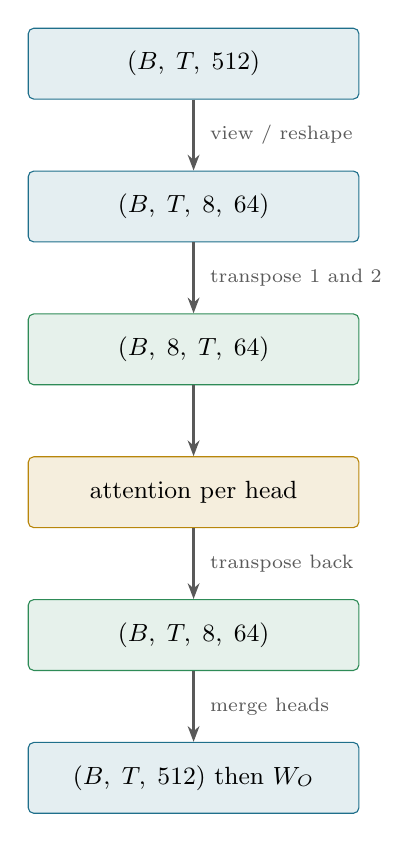
\begin{tikzpicture}[
  box/.style={rectangle,draw,rounded corners=2pt,minimum height=9mm,
              align=center,font=\small},
  arrow/.style={-{Stealth[length=2mm]},thick,gray!70!black}
]
\node[box,fill=hindiblue!12,draw=hindiblue,minimum width=42mm] (a) {$(B,\;T,\;512)$};
\node[box,fill=hindiblue!12,draw=hindiblue,minimum width=42mm,below=9mm of a] (b) {$(B,\;T,\;8,\;64)$};
\node[box,fill=conceptgreen!12,draw=conceptgreen,minimum width=42mm,below=9mm of b] (c) {$(B,\;8,\;T,\;64)$};
\node[box,fill=examplegold!14,draw=examplegold,minimum width=42mm,below=9mm of c] (d) {attention per head};
\node[box,fill=conceptgreen!12,draw=conceptgreen,minimum width=42mm,below=9mm of d] (e) {$(B,\;T,\;8,\;64)$};
\node[box,fill=hindiblue!12,draw=hindiblue,minimum width=42mm,below=9mm of e] (f) {$(B,\;T,\;512)$ then $W_O$};

\draw[arrow] (a) -- node[right,font=\scriptsize] {\;view / reshape} (b);
\draw[arrow] (b) -- node[right,font=\scriptsize] {\;transpose 1 and 2} (c);
\draw[arrow] (c) -- (d);
\draw[arrow] (d) -- node[right,font=\scriptsize] {\;transpose back} (e);
\draw[arrow] (e) -- node[right,font=\scriptsize] {\;merge heads} (f);
\end{tikzpicture}
\end{center}

\begin{saybox}
``The reshape is $(B,T,512) \rightarrow (B,T,8,64) \rightarrow (B,8,T,64)$, so
each head attends inside its own 64-dimensional subspace, then the exact inverse
to concatenate the heads back before the output projection $W_O$.''
\end{saybox}

\subsection{Why divide by $\sqrt{d_k}$}

\[
\mathrm{Attention}(Q,K,V) = \mathrm{softmax}\!\left(\frac{QK^{\top}}{\sqrt{d_k}} + M\right)V
\]

\begin{concept}{The scaling, explained simply}
Q and K entries are roughly zero-mean with variance about 1. A dot product adds
up $d_k = 64$ such products, so its variance is about 64 and its standard
deviation about 8.

Feeding numbers of size $\pm 8$ into softmax makes it almost one-hot: one value
gets essentially all the probability. And when softmax is saturated like that,
its gradient is almost zero, so learning stops.

Dividing by $\sqrt{d_k} = 8$ brings the scores back to roughly unit variance,
which keeps softmax in the range where it responds to changes.
\end{concept}

\subsection{The causal mask}

\begin{concept}{Why the mask exists}
The model is trained to predict the next token. If position 5 could see position
6, predicting position 6 would be trivial --- just copy. The model would score
perfectly during training and be useless at generation time, when the future
does not exist yet.

So we block it: position $t$ may attend only to positions $\le t$.
\end{concept}

The mask is an upper-triangular matrix of $-\infty$, added to the scores
\emph{before} softmax. It is stored as a buffer and sliced to \p{[:T,:T]}.

\begin{implementation}{Proving the mask works --- exactly}
The assignment asks to verify this empirically. My test
(\p{test\_causal\_mask\_blocks\_the\_future}) changes every token after position
$t$ and measures how much the logits at positions $\le t$ move.

The answer is \textbf{exactly 0.000e+00}. Not ``within tolerance''.
\end{implementation}

\begin{saybox}
``It is exactly zero, not approximately zero, because $\mathrm{softmax}(-\infty)$
is exactly $0$ and $0 \times v$ is exactly $0$ in floating point. The future
contributes literally nothing, not merely something small.''
\end{saybox}

\section{Step 4 --- The rest of the block}

\subsection{Feed-forward network}

Two linear layers with GELU in between: $512 \rightarrow 2048 \rightarrow 512$.

\begin{concept}{What the feed-forward layer is for}
Attention moves information \emph{between} positions. The feed-forward network
processes each position \emph{on its own}, with no mixing. It is where most of
the model's parameters live and where a lot of the actual ``knowledge'' is
stored. The wide middle layer (4$\times$) gives it room to compute something
non-linear before compressing back.
\end{concept}

\subsection{Residual connections}

\begin{concept}{Residual connections}
Instead of $x \rightarrow f(x)$, we do $x \rightarrow x + f(x)$. Each sublayer
\emph{adds} a correction rather than replacing everything.

This matters for training: during backpropagation the gradient has a direct path
straight through the additions back to layer 0, so it does not have to survive
being multiplied by six layers of weights. Without residuals, deep stacks simply
do not train.
\end{concept}

\subsection{Pre-norm vs post-norm}

I use \textbf{pre-norm}: LayerNorm is applied \emph{before} each sublayer, not
after.

\begin{concept}{Why pre-norm is more stable}
With post-norm, the residual path passes through a LayerNorm at every single
block, so the gradient gets rescaled six times on its way back. With pre-norm
the residual path is clean --- an unbroken sum from the output all the way to
the embedding.

Post-norm can be trained, but it needs careful learning-rate warmup and is
fragile in deep stacks. Pre-norm is what almost all modern models use.
\end{concept}

\subsection{LayerNorm}

\begin{concept}{LayerNorm in simple words}
For each position separately, take its 512 numbers, subtract their mean and
divide by their standard deviation, then scale and shift by learned parameters.

The effect is to keep the numbers flowing through the network in a consistent
range, so that no layer suddenly receives inputs that are a thousand times
bigger than it expects.
\end{concept}

\section{Step 5 --- Output and weight tying}

The final LayerNorm is followed by a linear layer mapping 512 to the vocabulary
size, giving one score per possible next token.

\begin{implementation}{Weight tying}
I reuse the \emph{input embedding matrix} as the output projection, transposed.
This saves $8{,}000 \times 512 = 4{,}096{,}000$ parameters --- about 15\% of
\MH.

The justification is that both matrices represent the same thing: a mapping
between tokens and vectors. There is no reason to learn that mapping twice.
\end{implementation}

\section{The training objective}

Cross-entropy between the logits at position $t$ and the actual token at
position $t+1$, averaged over all positions.

\begin{concept}{Cross-entropy, simply}
The model outputs a probability for every possible next token. Cross-entropy
is $-\log(\text{probability it gave to the correct token})$.

If it gave the right answer probability 1, the loss is 0. If it gave it
probability 0.01, the loss is about 4.6. So the loss punishes confident wrong
answers very heavily.
\end{concept}

\begin{implementation}{How the shift is done}
In my data loader, \p{x = stream[o : o+block\_size]} and
\p{y = stream[o+1 : o+1+block\_size]}. The targets are simply the inputs shifted
by one position. The model never sees its own target because of the causal mask.
\end{implementation}

\section{Dropout --- all four places}

The examiner asked about this. Name all four sites, all at $p = 0.1$:

\begin{enumerate}[leftmargin=*]
\item \textbf{Embedding dropout} --- on the summed token + position embedding,
      before the first block.
\item \textbf{Attention dropout} --- on the softmax \emph{probabilities}, after
      softmax and before multiplying by $V$.
\item \textbf{Residual dropout} --- on the attention output after $W_O$, before
      the residual addition.
\item \textbf{Feed-forward dropout} --- on the FFN output.
\end{enumerate}

\begin{concept}{What dropout does}
During training, dropout randomly sets a fraction of the numbers to zero. This
stops the model from relying too heavily on any one feature, because that
feature might not be there next time. It is a way of forcing redundancy, which
reduces overfitting.
\end{concept}

\begin{implementation}{Site 2 is the interesting one}
Dropping \emph{attention probabilities} is different from ordinary dropout. It
randomly cuts attention edges, so a head cannot stake everything on a single key
position. It regularises the \emph{routing} of information, not just the
features.

A detail worth knowing: after dropout the attention rows no longer sum to 1.
That is accepted. PyTorch uses ``inverted'' dropout, which scales the surviving
values by $1/(1-p)$ during training, so the \emph{expected} value is preserved.
\end{implementation}

\begin{warnbox}[Is dropout on during evaluation?]
\textbf{No.} \p{model.eval()} disables every \p{nn.Dropout}, and I call it before
validation, before \p{generate()}, and inside the attention tooling.

Because PyTorch uses inverted dropout, nothing needs rescaling at test time.

\medskip
\textbf{Likely follow-up:} ``what if you left it on?'' Perplexity would be
inflated \emph{and} non-deterministic --- a different random mask every pass, so
the same test set would give a different number each time. Every metric in my
report depends on \p{eval()} having been called.
\end{warnbox}

% =======================================================================
\chapter{Phase 2 --- Training}

\section{The settings, and why}

\begin{center}
\begin{tabular}{@{}ll@{}}
\toprule
\textbf{Setting} & \textbf{Value and reason} \\
\midrule
Optimiser & AdamW, $\beta = (0.9, 0.95)$ \\
Weight decay & 0.1, \emph{on matrices only} \\
Peak learning rate & $6 \times 10^{-4}$ \\
Minimum learning rate & $6 \times 10^{-5}$ \\
Warmup & 500 steps, then cosine decay \\
Effective batch & $32 \times 2 \times 512 = 32{,}768$ tokens per step \\
Precision & fp16 with GradScaler (T4 has no bf16) \\
Gradient clipping & 1.0 \\
\bottomrule
\end{tabular}
\end{center}

\begin{concept}{AdamW vs Adam}
Both adapt the learning rate per parameter. The difference is how weight decay
is applied.

In plain Adam, the L2 penalty is added into the gradient, and then gets divided
by the second-moment estimate along with everything else --- so parameters with
small gradients get \emph{more} decay. That is not what anybody wants.

AdamW ``decouples'' it: the decay is applied directly to the weights, separately
from the gradient step. That is the correct behaviour.
\end{concept}

\begin{implementation}{Decay on matrices only}
I apply weight decay only to 2-D parameters (the weight matrices). Biases,
LayerNorm gains and embeddings are excluded.

The reason: those parameters set \emph{scales and offsets}. They do not perform
the linear mixing that weight decay is meant to regularise, and shrinking them
toward zero hurts more than it helps.
\end{implementation}

\begin{concept}{Warmup and cosine decay}
At the very start, the model's weights are random and the Adam moment estimates
are meaningless. Taking a big step then can throw the model somewhere it never
recovers from. So warmup raises the learning rate linearly from almost zero over
the first 500 steps.

After that, cosine decay slowly lowers it. Large steps early explore; small
steps later settle into a good minimum.
\end{concept}

\begin{concept}{Gradient accumulation}
\p{batch\_size} is limited by how much fits in GPU memory. \p{grad\_accum\_steps}
lets me run several micro-batches and add up their gradients before taking one
optimiser step.

So the \emph{effective} batch is 32 sequences $\times$ 2 accumulation steps
$\times$ 512 tokens $=$ 32,768 tokens per update. Both models use exactly the
same number, so their token budgets match.
\end{concept}

\begin{concept}{fp16 and the GradScaler}
fp16 (16-bit floats) is faster and uses less memory, but it has a narrow
exponent range. Small gradients can underflow to zero and be lost.

The GradScaler multiplies the loss by a large factor before backpropagation, so
the gradients land in a representable range, then divides it out before the
optimiser step. bfloat16 does not need this because it has a wider exponent
range --- but the Tesla T4 (compute capability 7.5) does not support bfloat16.
\end{concept}

\section{What actually happened}

\begin{center}
\begin{tabular}{@{}lrr@{}}
\toprule
 & \textbf{Model H} & \textbf{Model L} \\
\midrule
Steps completed & 14,520 & 14,440 \\
Tokens seen & 475,791,360 & 473,169,920 \\
Wall clock on Tesla T4 & 11.0 h & 11.0 h \\
Throughput & $\sim$12.0k tokens/s & $\sim$12.0k tokens/s \\
Best checkpoint & step 14,500 & step 14,000 \\
\bottomrule
\end{tabular}
\end{center}

\section{Checkpoints and resume}

\begin{implementation}{What is inside a checkpoint}
\begin{itemize}
\item model weights
\item optimizer state (Adam's two moment estimates per parameter)
\item scheduler state
\item current step, tokens consumed, best validation loss
\item the full run configuration
\item \textbf{both RNG states} --- torch and numpy
\end{itemize}

Resume was verified across three consecutive sessions before the real runs
began.
\end{implementation}

\begin{concept}{Why the RNG states matter}
Most people forget these. Without them, a resumed run draws a different order of
training data and different dropout masks. The run still works, but it is no
longer the \emph{same experiment} --- and reproducibility is an explicit
requirement of the assignment.
\end{concept}

\begin{warnbox}[A real bug I found and fixed]
My learning-rate schedule originally restored its \emph{horizon}
(\p{max\_steps}) from the checkpoint.

When I resumed with a \emph{larger} \p{max\_steps} --- the normal case when a
session dies and you restart with a longer run --- the restored horizon left
\p{step > max\_steps}, which pinned the learning rate at its floor for the whole
extension. Training looked stalled and I nearly misdiagnosed it as a data
problem.

The fix: restore \emph{progress} only. The schedule's shape comes from the live
config.
\end{warnbox}

% =======================================================================
\chapter{Phase 2 --- Evaluation and What the Numbers Mean}

\section{Perplexity and bits-per-byte --- the headline}

\begin{center}
\begin{tabular}{@{}lrrl@{}}
\toprule
\textbf{Test metric} & \textbf{Model H} & \textbf{Model L} & \textbf{Winner} \\
\midrule
Cross-entropy (nats) & 3.3109 & 3.8433 & H \\
Perplexity & 27.41 & 46.68 & H, by 41\% \\
Bits-per-byte & 0.5382 & 0.4846 & L \\
Bytes per token & 8.875 & 11.441 & --- \\
\bottomrule
\end{tabular}
\end{center}

Both scored over 1,999,872 tokens per split.

\begin{concept}{Perplexity}
Perplexity is just $e^{\text{cross-entropy}}$. It has a nice interpretation: it
is roughly ``how many options is the model effectively choosing between at each
step''.

A perplexity of 27 means the model is about as uncertain as if it were picking
uniformly among 27 equally likely tokens.
\end{concept}

\begin{warnbox}[Why perplexity is unfair across different tokenizers]
Perplexity is measured \textbf{per token}. But a token is not a fixed amount of
text!

Nepali's tokens carry 11.44 bytes of text on average; Hindi's carry 8.88. So a
Nepali token is a \emph{bigger prediction} --- more text has to be guessed at
once. Of course it is harder.

Comparing perplexity across two different tokenizers is like comparing ``errors
per page'' between a book with 200 words per page and one with 500.
\end{warnbox}

\begin{concept}{Bits-per-byte fixes this}
Bits-per-byte divides the total information cost by the number of \emph{UTF-8
bytes} of the original text, not by the number of tokens. Bytes are the same
unit for both languages, so the tokenizer disappears from the denominator.
\end{concept}

\textbf{Be able to derive it live.} This is the most impressive twenty seconds
available to you in the room:

\[
\mathrm{BPB} = \frac{\mathrm{CE}_{\text{nats}}}{\ln 2 \times \text{bytes per token}}
\]
\[
\text{Model H:}\quad \frac{3.3109}{0.6931 \times 8.875} = 0.5382
\qquad
\text{Model L:}\quad \frac{3.8433}{0.6931 \times 11.441} = 0.4846
\]

\begin{saybox}
``Both numbers are correct; they measure different things. Nepali's BPE packs
11.44 bytes into a token against Hindi's 8.88, so its tokens are individually
harder to predict but each one carries more text. Normalising by UTF-8 bytes
takes the tokenizer out of the denominator --- and then the gap almost vanishes
and actually reverses.

Reporting perplexity alone would have supported the conclusion that the
low-resource model is much worse. It is not.''
\end{saybox}

\section{Generation quality and the temperature question}

\begin{concept}{Temperature}
When the model generates text, it produces a score for every possible next
token. Temperature divides those scores before turning them into probabilities:
\[
P(\text{token}) = \mathrm{softmax}(\text{logits} / T)
\]
$T \rightarrow 0$ means always take the highest score (greedy). Large $T$ makes
everything nearly equally likely (random).
\end{concept}

\begin{center}
\begin{tabular}{@{}lrrrr@{}}
\toprule
\textbf{Model H setting} & \textbf{Repetition} & \textbf{Distinct-1} & \textbf{BLEU-4} & \textbf{chrF++} \\
\midrule
greedy & 0.598 & 0.172 & 1.96 & 12.49 \\
$T = 0.5$ & 0.212 & 0.275 & 1.80 & 14.33 \\
$T = 1.0$ & \textbf{0.002} & 0.520 & 1.01 & \textbf{16.29} \\
$T = 1.5$ & 0.000 & 0.702 & 0.16 & 14.67 \\
\midrule
\textbf{Model L setting} & & & & \\
\midrule
greedy & 0.577 & 0.179 & 2.37 & 14.48 \\
$T = 0.5$ & 0.190 & 0.345 & 1.88 & 16.54 \\
$T = 1.0$ & \textbf{0.001} & 0.634 & 1.69 & \textbf{18.05} \\
$T = 1.5$ & 0.000 & 0.793 & 0.78 & 16.13 \\
\bottomrule
\end{tabular}
\end{center}

\begin{center}
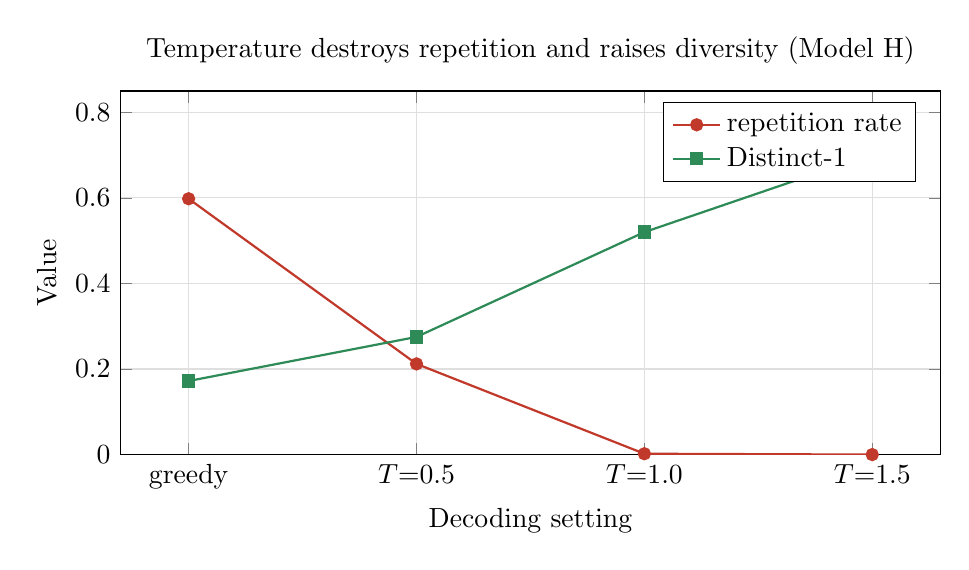
\begin{tikzpicture}
\begin{axis}[
  width=12cm,height=6.2cm,
  xlabel={Decoding setting},
  ylabel={Value},
  xtick={0,1,2,3},
  xticklabels={greedy,$T{=}0.5$,$T{=}1.0$,$T{=}1.5$},
  ymin=0,ymax=0.85,
  legend pos=north east,
  legend cell align={left},
  grid=major,grid style={gray!25},
  title={Temperature destroys repetition and raises diversity (Model H)}
]
\addplot[color=warnred,mark=*,thick] coordinates {(0,0.598)(1,0.212)(2,0.002)(3,0.000)};
\addlegendentry{repetition rate}
\addplot[color=conceptgreen,mark=square*,thick] coordinates {(0,0.172)(1,0.275)(2,0.520)(3,0.702)};
\addlegendentry{Distinct-1}
\end{axis}
\end{tikzpicture}
\end{center}

\begin{concept}{Why low temperature causes repetition loops}
At low temperature the highest-scoring token always wins. So if the model ever
returns to a state it has been in before, it produces exactly the same
continuation --- and then returns to that state again. It is a deterministic
loop with nothing random to break it.

Raising the temperature introduces enough randomness to escape.
\end{concept}

\begin{saybox}
``Greedy decoding \emph{degenerates} --- 59.8\% of generated 4-grams are repeats
and the samples visibly loop. Raising temperature monotonically destroys that
repetition, down to 0.2\% at $T=1.0$. Model L behaves identically: 0.577 down to
0.001.''
\end{saybox}

\subsection{The subtle part --- BLEU and chrF++ disagree}

\begin{itemize}
\item \textbf{BLEU falls monotonically} (1.96 $\rightarrow$ 0.16). BLEU counts
      exact n-gram matches against one reference. Greedy's repeated common
      n-grams accidentally match, so BLEU actually \emph{rewards} the degenerate
      output.
\item \textbf{chrF++ peaks at $T = 1.0$} (16.29 for H, 18.05 for L). chrF++
      scores \emph{character} n-grams, so it gives credit for correct Devanagari
      morphology even when the exact words differ from the reference.
\end{itemize}

\begin{saybox}
``$T=1.0$ removes the repetition \emph{and} peaks chrF++, so diversity costs no
fidelity up to that point. It also shows why BLEU is a poor metric for
open-ended generation in a morphologically rich language --- a degenerate loop
can outscore a fluent continuation.''
\end{saybox}

\begin{implementation}{Why I wrote ROUGE-L myself}
The standard \p{rouge\_score} package strips non-ASCII characters, which zeroes
out Devanagari completely --- every score would have been 0.0.

Mine is a longest-common-subsequence over whitespace tokens.
\end{implementation}

\section{Attention analysis}

\begin{center}
\begin{tabular}{@{}lrr@{}}
\toprule
Phase 2, $T = 512$, uniform baseline 5.2565 nats & \textbf{Model H} & \textbf{Model L} \\
\midrule
Mean attention entropy & 3.205 & 3.090 \\
Mean attention distance & 62.36 & 54.51 \\
Previous-token head (layer 3) & 0.06 nats @ 1.3 & 0.14 nats @ 1.1 \\
\bottomrule
\end{tabular}
\end{center}

\begin{concept}{Attention entropy}
Entropy measures how spread out a probability distribution is. Low entropy means
the head is focused on one or two positions. High entropy means it is spread
thinly over everything.

The ``uniform baseline'' is what the entropy would be if a head attended equally
to everything it is allowed to see. Being far below the baseline proves the
model learned structure rather than just averaging.
\end{concept}

\begin{warnbox}[If they ask where 5.2565 comes from]
It is \textbf{not} $\ln(512) = 6.24$.

Under causal masking, query position $t$ can only see $t+1$ keys. So the entropy
of uniform attention at that position is $\ln(t+1)$, which is small at the start
of the sequence and large at the end.

The baseline is the \textbf{mean of $\ln(t+1)$ over all positions}, which for
$T = 512$ comes to 5.2565.
\end{warnbox}

\begin{concept}{Mean attention distance}
For each query position, how far back does it look on average? A head with
distance 1.3 is looking at the immediately preceding token. A head with distance
62 is looking far back across the sequence.
\end{concept}

\begin{saybox}
``Both models --- different languages, different tokenizers, different seeds ---
\textbf{independently converged on a previous-token head at layer 3}: entropy
0.06 at distance 1.3 for H, 0.14 at 1.1 for L. Nobody designed that. And mean
entropy sits about 2 nats below the uniform baseline, so attention is genuinely
structured, not diffuse.''
\end{saybox}

\subsection{Reading a heatmap out loud}

Point at three things, in this order:

\begin{enumerate}[leftmargin=*]
\item \textbf{The upper triangle is uniformly zero.} That is the causal mask,
      visually --- the same fact the test proves numerically.
\item \textbf{The bright first column} --- an ``attention sink'' at position 0.
      Softmax must sum to 1, so when a head has nothing specific to attend to it
      parks probability mass on the first token.
\item \textbf{The tight diagonal band} in early layers means local, positional
      heads. Late layers show off-diagonal structure that follows content.
\end{enumerate}

% =======================================================================
\chapter{Phase 3 --- The Reasoning Dataset}

\section{What the assignment asked for}

Build \emph{my own} synthetic dataset of comparison and transitive-reasoning
questions, in each model's own language, generated programmatically so that
every correct answer is known by construction. Do not download an existing
benchmark.

\section{The four task families}

\begin{center}
\begin{tabular}{@{}llll@{}}
\toprule
\textbf{Family} & \textbf{Hops} & \textbf{Candidates} & \textbf{Example (Hindi)} \\
\midrule
\p{compare2} & 1 & 2 & \dn{विजय सोहन से धीमा है। दोनों में से तेज़ कौन है?} \\
\p{transitive3} & 2 & 3 & \dn{मीना प्रीति से छोटी है। प्रीति सुनीता से छोटी है।} \\
\p{numeric2} & 1 & 2 & \dn{संगीता की उम्र १३ साल है। रेखा की उम्र ६८ साल है।} \\
\p{numeric3} & 1 & 3 & three measured values, pick the extreme \\
\bottomrule
\end{tabular}
\end{center}

Five comparable attributes: height, age, weight, speed and wealth. The last two
have no natural numeric phrasing in either language, so they appear only in the
comparison tasks.

\begin{implementation}{Direction variation}
Both the \emph{stated} direction and the \emph{asked} direction vary
independently. If the sentence says ``A is taller than B'' and the question asks
who is \emph{shorter}, the answer is B.

Without this the answer would simply always be the first-named entity. Measured:
the answer is the first-named entity in 46\% of examples --- i.e. chance.
\end{implementation}

\section{Size and leakage control}

\begin{center}
\begin{tabular}{@{}lrrr@{}}
\toprule
\textbf{Split} & \textbf{Examples} & \textbf{Templates} & \textbf{Entity names} \\
\midrule
train & 20,000 & 14 & 40 \\
validation & 2,000 & 4 & 10 \\
test & 2,000 & 4 & 10 \\
\bottomrule
\end{tabular}
\end{center}

Identical for both languages, and the two corpora share \textbf{no sentence, no
entity name and no template} --- verified programmatically.

\begin{concept}{Train--test leakage in a synthetic dataset}
If I generate 20,000 training examples and 2,000 test examples from the same
pool of names and the same sentence templates, the model can score well by
memorising ``this name goes with this answer'' or ``this phrasing means that''.
The test score would then measure memorisation, not reasoning.
\end{concept}

\begin{implementation}{Both defences, applied together}
\begin{itemize}
\item \textbf{Held-out entity names} --- 40 / 10 / 10, disjoint. A test question
      is always about people the model never saw in training.
\item \textbf{Held-out templates} --- 14 / 4 / 4, disjoint. A test question is
      always phrased in a way the model never saw either.
\end{itemize}

The generator \textbf{asserts} this rather than assuming it: if the pools ever
overlap, it crashes instead of quietly inflating the test score.
\end{implementation}

This paid off directly --- see Section~\ref{sec:offprompt}.

\section{Two defects I caught in my own dataset}

Volunteer these. They show you reviewed your own work adversarially.

\subsection{A 45\% gender-agreement leak}

\begin{warnbox}[The bug]
Hindi adjectives inflect for gender: \dn{छोटा} for a man, \dn{छोटी} for a woman.

So a question ending \dn{सबसे छोटी कौन है?} asked about one woman and two men
has exactly \emph{one grammatically possible answer} --- the woman. A model
could score well by matching grammatical agreement and never perform the
comparison at all.

\textbf{181 out of 400 examples --- 45\% --- were solvable this way.}
\end{warnbox}

\textbf{The fix:} draw every entity in an example from the \emph{same} gender.
Then the adjective carries no information about which entity is meant, and the
answer can only come from the comparison. Verified: zero mixed-gender examples.

\subsection{Nepali numerals were completely unrepresentable}
\label{sec:digits}

\begin{warnbox}[The bug]
\ML's BPE vocabulary contains \textbf{no Devanagari digit at all} --- not one of
\dn{०१२३४५६७८९} is a vocabulary piece --- and it was trained \emph{without byte
fallback}.

So every Devanagari numeral encoded to \p{<unk>}. My first draft ran a
\textbf{4.8\% unknown-token rate} across the whole finetuning corpus, which
would have trained Model L on holes exactly where the quantities belong.
\end{warnbox}

\textbf{The fix:} the Nepali generator writes numerals with Arabic digits
(\p{141}, \p{175}), which the vocabulary covers completely and which modern
Nepali prose overwhelmingly uses anyway. Model H's Unigram vocabulary covers
\emph{both} digit systems at zero unknowns, so Hindi keeps Devanagari digits.

\begin{saybox}
``The asymmetry between the two generators is not an inconsistency. It is the
low-resource tokenizer's coverage gap showing up in practice, and I report it as
a finding rather than papering over it. Both corpora now tokenize at exactly
0.000000 unknown rate.''
\end{saybox}

\section{Natural phrasing in Nepali}

The assignment requires the target language's script \emph{and} natural
phrasing. In Nepali the comparative postposition and the genitive attach to the
preceding word:

\begin{center}
\dn{रबिनको उचाइ 141 सेन्टिमिटर छ।} \quad and \quad \dn{कल्पनाभन्दा}
\end{center}

Writing them detached (\dn{रबिन को}, \dn{कल्पना भन्दा}) is the usual signature of
Nepali that has been translated from Hindi. My templates attach them.

% =======================================================================
\chapter{Phase 3 --- Finetuning}

\section{The protocol}

\begin{implementation}{Every rule of the specified protocol}
\begin{itemize}
\item Each model starts from \textbf{its own} Phase 2 checkpoint --- H from step
      14,500, L from step 14,000. Never the other model, never from scratch.
\item Each keeps \textbf{its own} Phase 1 tokenizer, so the embedding and output
      matrices keep their pretrained rows. The finetuner \textbf{asserts} that
      the tokenizer's vocabulary size matches the checkpoint rather than
      trusting the config file.
\item Checkpoints use the same resume-capable format as pretraining, which is
      what lets the Phase 2 evaluation and attention tools load them unchanged.
\end{itemize}
\end{implementation}

\section{Hyperparameters --- identical for both models}

\begin{center}
\begin{tabular}{@{}lll@{}}
\toprule
\textbf{Setting} & \textbf{Value} & \textbf{Why} \\
\midrule
Peak learning rate & $6 \times 10^{-5}$ & one tenth of the pretraining peak \\
Minimum LR & $6 \times 10^{-6}$ & cosine floor \\
Warmup & 100 steps & \\
Batch size & 32 examples & \\
Epochs & 2 (1,250 steps) & \\
Optimiser & AdamW, $\beta=(0.9,0.95)$, wd 0.1 & matrices only \\
Gradient clip & 1.0 & \\
Precision & fp16 + GradScaler & T4 has no bf16 \\
Evaluation & every 20 steps & \\
Loss & \textbf{answer tokens only} & \\
\bottomrule
\end{tabular}
\end{center}

\begin{concept}{Why a much smaller learning rate for finetuning}
The model already contains a language model worth keeping. A pretraining-sized
step would overwrite that knowledge before the new task is learned.

The classic failure mode is a model that answers in the right \emph{format} but
has forgotten how to read the question. One tenth of the pretraining peak is a
standard, conservative choice.
\end{concept}

\section{Two design decisions worth explaining}

\subsection{Loss on the answer only}

\begin{implementation}{How it works}
Prompt target positions are set to $-1$, and the model's
\p{cross\_entropy(..., ignore\_index=-1)} already skips those.

If I trained on the prompt too, most of the gradient would go into reproducing
question templates --- which the model is \emph{given for free} at test time ---
and the thing actually being measured (can it name the right entity) would get
only a small share of the signal.
\end{implementation}

\subsection{Bucketing by prompt length instead of padding}

\begin{concept}{Why padding would break things here}
My models use \emph{learned absolute} positional embeddings, so a token's
representation depends on its index in the sequence.

If I pad on the \emph{left}, every real token shifts to a position it never
occupied during pretraining --- the model sees them in the wrong place.

If I pad on the \emph{right}, training is fine, but generation breaks, because
generation appends new tokens at the end and the padding is in the way.

\textbf{The solution:} group examples whose prompts tokenize to exactly the same
length. Then every sequence in a batch is genuinely aligned and no padding is
needed in the prompt at all.
\end{concept}

\section{What happened during training}

\begin{center}
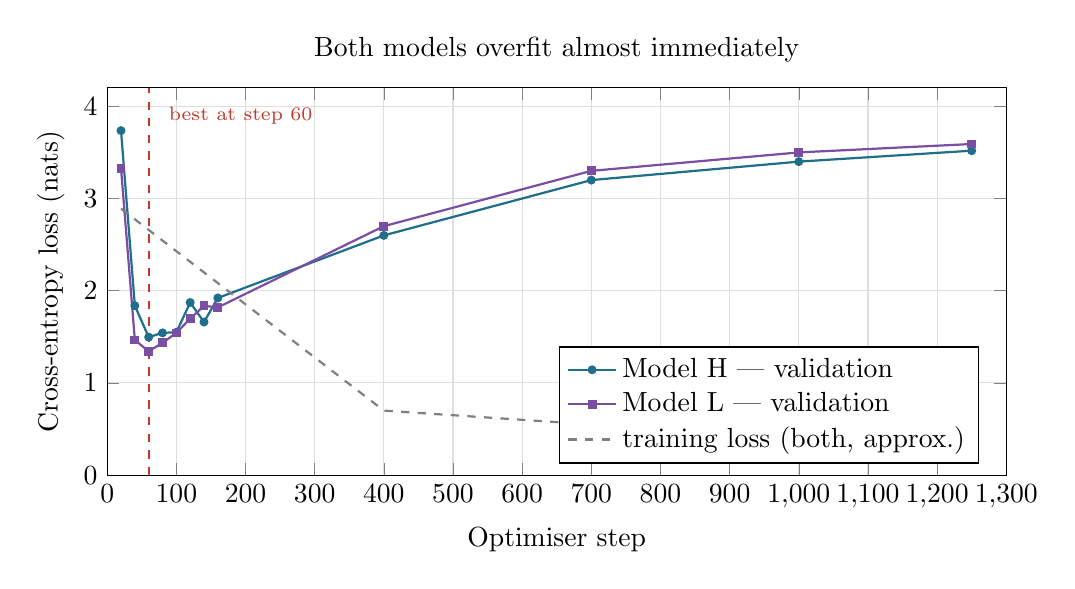
\begin{tikzpicture}
\begin{axis}[
  width=13cm,height=6.5cm,
  xlabel={Optimiser step},
  ylabel={Cross-entropy loss (nats)},
  xmin=0,xmax=1300,ymin=0,ymax=4.2,
  legend pos=south east,
  legend cell align={left},
  grid=major,grid style={gray!25},
  title={Both models overfit almost immediately}
]
\addplot[color=hindiblue,mark=*,mark size=1.2pt,thick] coordinates {
(20,3.7361)(40,1.8377)(60,1.4966)(80,1.5432)(100,1.5496)(120,1.8722)
(140,1.6604)(160,1.9217)(400,2.6)(700,3.2)(1000,3.4)(1250,3.5188)};
\addlegendentry{Model H --- validation}
\addplot[color=nepalipurple,mark=square*,mark size=1.2pt,thick] coordinates {
(20,3.3294)(40,1.4653)(60,1.3427)(80,1.4356)(100,1.5423)(120,1.6975)
(140,1.8362)(160,1.8193)(400,2.7)(700,3.3)(1000,3.5)(1250,3.5911)};
\addlegendentry{Model L --- validation}
\addplot[color=gray,dashed,thick] coordinates {(20,2.89)(400,0.7)(800,0.5)(1250,0.44)};
\addlegendentry{training loss (both, approx.)}
\draw[warnred,thick,dashed] (axis cs:60,0) -- (axis cs:60,4.2);
\node[warnred,font=\scriptsize,anchor=west] at (axis cs:75,3.9) {best at step 60};
\end{axis}
\end{tikzpicture}
\end{center}

\begin{center}
\begin{tabular}{@{}lrr@{}}
\toprule
 & \textbf{Model H} & \textbf{Model L} \\
\midrule
Best validation loss & 1.4966 & 1.3427 \\
Step of best & \textbf{60} & \textbf{60} \\
Validation loss at step 1,250 & 3.5188 & 3.5911 \\
Training loss at step 1,250 & 0.44 & 0.60 \\
\bottomrule
\end{tabular}
\end{center}

\begin{concept}{What overfitting looks like, and why it happened here}
Overfitting is when the model keeps getting better on the data it is trained on
while getting \emph{worse} on data it has not seen. The two curves separate.

Here it happened extremely fast --- by step 60. The reason is the dataset
design: with only 40 training names and 14 templates, memorising ``the answer is
usually one of these 40 names'' is much easier than learning to read the
question and copy the right name out of it.

Saving on \emph{best validation loss} is what kept the evaluated checkpoints
usable. Otherwise I would have reported the badly overfit final model.
\end{concept}

\begin{warnbox}[A methodology mistake I found and fixed]
My first run evaluated every \textbf{100} steps, and its best validation loss
landed at step 100 --- which is also exactly where warmup ends and the learning
rate first reaches its peak. The checkpoint was being selected from a grid too
coarse to find the real optimum.

Re-running with a \textbf{20}-step grid, changing nothing else, moved Model L
from \textbf{14.90\% to 29.45\%} exact match and Model H from 32.70\% to
35.15\%.

The conclusions did not change --- but the numbers did, and the coarse grid
would have understated both models.
\end{warnbox}

% =======================================================================
\chapter{Phase 3 --- Results and What They Really Mean}

\section{Why I report two metrics}

\begin{warnbox}[The problem with exact match alone]
A \emph{pretrained} model has never seen this prompt format. It will not
spontaneously answer with a bare name. So its exact match is 0\% --- and that
0\% is a \textbf{floor artefact}, not a measurement of reasoning ability.

Comparing ``0\% before'' to ``35\% after'' therefore tells you the model learned
the output format. It tells you nothing about whether it learned to compare.
\end{warnbox}

\begin{concept}{Forced choice --- the fair test}
Instead of letting the model generate freely, I give it the entities the
question actually names as candidates. For each candidate I append it to the
prompt and compute the model's mean log-probability per answer token. The
highest-scoring candidate is taken as the model's answer.

Now chance is \emph{known}: with 2 candidates it is 50\%, with 3 it is 33.3\%.
Averaged over my test set it is \textbf{41.67\%}. So the pretrained baseline
becomes interpretable rather than a floor.
\end{concept}

\begin{implementation}{Why length-normalised}
Names tokenize into different numbers of pieces. Without dividing by the token
count, a one-token name beats a three-token name on \emph{total}
log-probability, for reasons that have nothing to do with the question.
\end{implementation}

\section{The headline table}

\begin{center}
\begin{tabular}{@{}llrrr@{}}
\toprule
\textbf{Model} & \textbf{Metric} & \textbf{Pretrained} & \textbf{Finetuned} & \textbf{Change} \\
\midrule
H & Exact match & 0.00\% & \textbf{35.15\%} & $+35.15$ \\
H & Forced choice & 39.80\% & 36.35\% & $-3.45$ \\
H & Answer-token loss & 5.2439 & \textbf{0.9408} & $-4.3031$ \\
\midrule
L & Exact match & 0.00\% & \textbf{29.45\%} & $+29.45$ \\
L & Forced choice & 38.80\% & 39.30\% & $+0.50$ \\
L & Answer-token loss & 5.5367 & \textbf{1.4351} & $-4.1016$ \\
\midrule
\multicolumn{2}{l}{\emph{forced-choice chance rate}} & \emph{41.67\%} & \emph{41.67\%} & --- \\
\bottomrule
\end{tabular}
\end{center}

\begin{saybox}
``Exact match went from 0\% to 35\%, which looks like success. It is not. On a
forced choice between the entities the question actually names, both models are
\textbf{at or below the 41.67\% chance rate}. Finetuning taught the output
format, not the comparison.''
\end{saybox}

\section{Per task family --- the agreement with chance}

\begin{center}
\begin{tabular}{@{}llrrrr@{}}
\toprule
\textbf{Model} & \textbf{Family} & \textbf{Cands} & \textbf{Chance} & \textbf{Pretrained} & \textbf{Finetuned} \\
\midrule
H & \p{compare2} & 2 & 50.0\% & 0.00\% & 47.40\% \\
H & \p{numeric2} & 2 & 50.0\% & 0.00\% & 47.40\% \\
H & \p{numeric3} & 3 & 33.3\% & 0.00\% & 33.40\% \\
H & \p{transitive3} & 3 & 33.3\% & 0.00\% & \textbf{12.40\%} \\
\midrule
L & \p{compare2} & 2 & 50.0\% & 0.00\% & 40.20\% \\
L & \p{numeric2} & 2 & 50.0\% & 0.00\% & 38.00\% \\
L & \p{numeric3} & 3 & 33.3\% & 0.00\% & 26.20\% \\
L & \p{transitive3} & 3 & 33.3\% & 0.00\% & \textbf{13.40\%} \\
\bottomrule
\end{tabular}
\end{center}

Model H's one-hop scores sit within 2.6 points of chance, and \p{numeric3} within
\textbf{0.1} points. The two-hop family is the only exception --- and it is
\emph{below} chance for both models.

\section{Why the two-hop task scores below chance}

This is the best answer in the whole project. It is a \emph{diagnosed} failure,
not a shrug.

\begin{center}
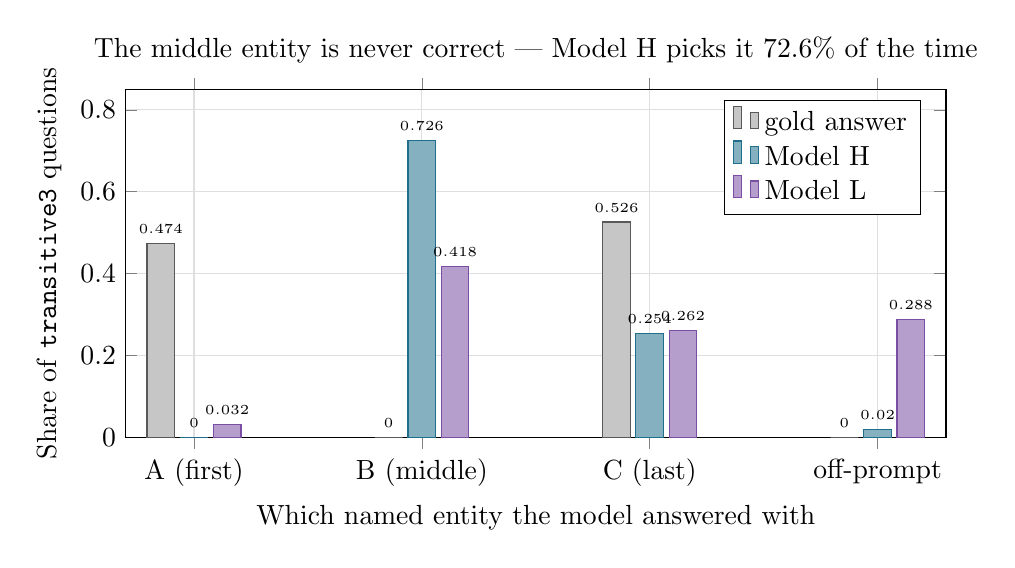
\begin{tikzpicture}
\begin{axis}[
  ybar,
  width=12cm,height=6cm,
  bar width=10pt,
  xlabel={Which named entity the model answered with},
  ylabel={Share of \texttt{transitive3} questions},
  symbolic x coords={A (first),B (middle),C (last),off-prompt},
  xtick=data,
  ymin=0,ymax=0.85,
  legend pos=north east,
  legend cell align={left},
  grid=major,grid style={gray!25},
  nodes near coords,
  every node near coord/.append style={font=\tiny,/pgf/number format/fixed,
        /pgf/number format/precision=3},
  title={The middle entity is never correct --- Model H picks it 72.6\% of the time}
]
\addplot[fill=gray!45,draw=gray!70!black] coordinates {(A (first),0.474)(B (middle),0.0)(C (last),0.526)(off-prompt,0.0)};
\addlegendentry{gold answer}
\addplot[fill=hindiblue!55,draw=hindiblue] coordinates {(A (first),0.0)(B (middle),0.726)(C (last),0.254)(off-prompt,0.020)};
\addlegendentry{Model H}
\addplot[fill=nepalipurple!55,draw=nepalipurple] coordinates {(A (first),0.032)(B (middle),0.418)(C (last),0.262)(off-prompt,0.288)};
\addlegendentry{Model L}
\end{axis}
\end{tikzpicture}
\end{center}

\begin{saybox}
``The chain is stated as \emph{A $>$ B, B $>$ C}, so the two extremes are always
A and C and the middle entity is \textbf{never} the correct answer. Model H
answers with the middle entity 72.6\% of the time and with A \textbf{0.0\%} of
the time.

B is the only name mentioned \emph{twice}. The model is selecting on salience
instead of following the inequality. That is exactly why it scores below random
guessing --- random would at least hit A and C sometimes.''
\end{saybox}

\section{One-hop answers show a recency bias}

\begin{center}
\begin{tabular}{@{}lrrr@{}}
\toprule
\textbf{Model H family} & \textbf{Answered first} & \textbf{Answered second} & \textbf{Gold split} \\
\midrule
\p{compare2} & 30.8\% & \textbf{62.0\%} & 48 / 52 \\
\p{numeric2} & 35.0\% & \textbf{65.0\%} & 50 / 50 \\
\bottomrule
\end{tabular}
\end{center}

Against a balanced gold distribution, Model H prefers the \emph{second-named}
entity roughly two to one. The failures show it plainly --- each of these is the
model answering with the most recently mentioned name:

\begin{example}{Model H recency failures}
\dn{ध्यान दीजिए: नवीन वरुण से अमीर है। अमीर कौन है?} \\
$\rightarrow$ model said \dn{वरुण}, correct answer \dn{नवीन}

\medskip
\dn{ध्यान दीजिए: अरुण नवीन से बड़ा है। बड़ा कौन है?} \\
$\rightarrow$ model said \dn{नवीन}, correct answer \dn{अरुण}
\end{example}

\section{Model L is much less grounded in the prompt}
\label{sec:offprompt}

\begin{center}
\begin{tabular}{@{}lrr@{}}
\toprule
\textbf{Answered with a name not in the question} & \textbf{Model H} & \textbf{Model L} \\
\midrule
\p{compare2} & 7.2\% & \textbf{19.2\%} \\
\p{numeric2} & 0.0\% & \textbf{25.0\%} \\
\p{numeric3} & 1.0\% & \textbf{21.2\%} \\
\p{transitive3} & 2.0\% & \textbf{28.8\%} \\
\bottomrule
\end{tabular}
\end{center}

Model L emits a memorised \emph{training} name --- repeatedly \dn{सिर्जना} ---
instead of one of the candidates in front of it. Model H does this too, but far
less (\dn{महेश}).

Both \emph{pretrained} models do it 100\% of the time (99.6\% for H on
\p{transitive3}).

\begin{saybox}
``Finetuning moved Model H almost entirely onto the prompt and Model L only
about three-quarters of the way. This is the single clearest resource-tier
difference in the phase --- and the held-out name pools are what make it
measurable at all. Without disjoint pools this behaviour would have scored as
partial success.''
\end{saybox}

\section{Successes}

The models do get questions right, including ones needing the direction flip:

\begin{example}{Correct answers}
\dn{ध्यान दीजिए: प्रवीण वरुण से हल्का है। भारी कौन है?} $\rightarrow$ \dn{वरुण} \checkmark

\medskip
\dn{ध्यान दीजिए: वरुण प्रवीण से गरीब है। अमीर कौन है?} $\rightarrow$ \dn{प्रवीण} \checkmark

\medskip
\dn{ध्यान दिनुहोस्: निरु कल्पनाभन्दा धनी छ। धनी को हो?} $\rightarrow$ \dn{निरु} \checkmark
\end{example}

\begin{warnbox}[Be honest about these]
Given the positional biases above, these are best read as the positional habit
\emph{coinciding} with the correct answer, rather than as evidence of genuine
comparison. Say that yourself before the examiner says it.
\end{warnbox}

% =======================================================================
\chapter{Phase 3 --- Attention After Finetuning}

\section{The method, and why it is fair}

\begin{implementation}{Three controls}
\begin{itemize}
\item Both checkpoints run on the \textbf{same} prompts. Attention entropy
      depends heavily on what is being attended to, so different text would
      confuse a finetuning effect with a text effect.
\item Prompts come from the reasoning \textbf{test} split --- held-out names,
      held-out templates --- so neither checkpoint has memorised them.
\item Every prompt in a batch has the \textbf{same token count}. Mean attention
      distance is measured in positions and the entropy baseline is $\ln(t)$, so
      both grow with sequence length. Comparing a 20-token prompt against a
      40-token one would show a difference that is purely arithmetic.
\end{itemize}
\end{implementation}

\section{Results}

\begin{center}
\begin{tabular}{@{}llrrr@{}}
\toprule
\textbf{Model} & \textbf{Checkpoint} & \textbf{Mean entropy} & \textbf{Mean distance} & \textbf{Baseline} \\
\midrule
H & pretrained & 1.9102 & 10.303 & 2.9545 ($T=46$) \\
H & finetuned & 1.8691 & 10.360 & \\
L & pretrained & 1.8327 & 9.415 & 2.8061 ($T=39$) \\
L & finetuned & 1.7833 & 10.158 & \\
\bottomrule
\end{tabular}
\end{center}

Finetuning made attention \textbf{sharper and longer-range at the same time} in
both models. Model L's mean distance rises 0.74 positions on a 39-token prompt
--- the model that most needed to learn to look at the prompt moved the most.

\subsection{Per-head shifts}

Layer means hide what actually happened. Finetuning a small model for a narrow
task moves a \emph{few} heads sharply rather than shifting every head slightly.

\begin{center}
\begin{tabular}{@{}llrr@{}}
\toprule
\textbf{Model} & \textbf{Head} & \textbf{$\Delta$ entropy} & \textbf{$\Delta$ distance} \\
\midrule
H & L1H5 & $-0.2734$ & $+1.257$ \\
H & L3H1 & $-0.2306$ & $\mathbf{+2.585}$ \\
H & L4H3 & $-0.2285$ & $+0.869$ \\
H & L4H1 & --- & $-1.367$ \\
\midrule
L & L1H3 & $-0.3336$ & $+1.836$ \\
L & L5H5 & $-0.3323$ & $+2.247$ \\
L & L2H6 & $-0.3062$ & $+1.412$ \\
L & L3H3 & --- & $\mathbf{+3.711}$ \\
\bottomrule
\end{tabular}
\end{center}

The pattern is consistent: the heads that changed most became \textbf{sharper
and longer-range simultaneously}. Middle layers (1--3) dominate the list in both
models --- which is where Phase 2 found the previous-token heads. Finetuning
appears to have repurposed part of that machinery to look further back for a
name.

\begin{warnbox}[Do not overclaim]
The shifts are real but \emph{small}, and accuracy did not improve.

The defensible reading: finetuning changed \textbf{where} the model looks
without giving it the mechanism to \emph{use} what it finds. It learned to reach
back for a name, but not \emph{which} name.

Also say plainly: this analysis is \textbf{correlational}. It shows which heads
moved; it does not prove those heads carry the comparison. The direct test would
be to ablate L3H1 or L3H3 and re-score.
\end{warnbox}

% =======================================================================
\chapter{The Question Bank}
\label{ch:bank}

Organised by what the Phase 1--2 examiner actually did: open the code, ask why,
then make you read a figure.

\section{On the code}

\begin{qabox}{Walk me through the forward pass.}
Answer in tensor shapes, not adjectives. See the listing on page
\pageref{ch:cheat} onward. The three reshapes are the part they are listening
for: $(B,T,512) \rightarrow (B,T,8,64) \rightarrow (B,8,T,64)$ and back.
\end{qabox}

\begin{qabox}{Show me the causal mask actually works.}
``My test perturbs every token after position $t$ and measures the change in
logits at positions $\le t$. It is \textbf{exactly 0.000e+00} --- not within
tolerance --- because $\mathrm{softmax}(-\infty)$ is exactly zero and
$0 \times v$ is exactly zero.''
\end{qabox}

\begin{qabox}{Why divide by $\sqrt{d_k}$?}
``Dot products over 64 dimensions have standard deviation about 8. Numbers that
large saturate softmax into a near one-hot distribution, and a saturated softmax
has almost no gradient. Dividing by $\sqrt{d_k}$ restores unit variance and
keeps softmax responsive.''
\end{qabox}

\begin{qabox}{What is in a checkpoint?}
Weights, optimizer state, scheduler state, step, tokens seen, best validation
loss, the full config, and both RNG states. Resume verified across three
sessions.
\end{qabox}

\begin{qabox}{Why a different tokenizer for each language?}
``Vocabularies are never shared --- that is a hard constraint. Each size was
chosen from that language's own measurements: fertility and unknown rate on
held-out text, traded against the embedding budget, where every extra 1,000
entries costs 512,000 parameters out of a 25M budget.''
\end{qabox}

\section{On the data}

\begin{qabox}{How did you split train / validation / test?}
``At the \textbf{document level}, with a fixed seed, roughly 96/2/2 for Hindi.
Document level is the point --- splitting after chunking would put two pieces of
the same article in train and test, and the test perplexity would be measuring
memorisation. \p{validate\_phase1.py} confirms zero overlap.''
\end{qabox}

\begin{qabox}{What were your cleaning steps?}
NFC normalise $\rightarrow$ strip zero-width and control characters $\rightarrow$
strip pure-Latin tokens $\rightarrow$ drop malformed / too short / low-Devanagari
/ wrong-language $\rightarrow$ deduplicate. 95.9\% character retention for Hindi.
Nepali adds a perplexity filter and MinHash/LSH dedup.
\end{qabox}

\begin{qabox}{Why NFC specifically?}
``Devanagari can be encoded precomposed or decomposed --- same visible string,
different bytes. Without normalising first, deduplication misses real duplicates
and the tokenizer learns two pieces for one grapheme.''
\end{qabox}

\section{On architecture choices}

\begin{qabox}{What positional encoding, and why not RoPE?}
See Section~\ref{sec:rope}. Never claim RoPE. Explain that it rotates Q and K
inside attention so scores depend on $i-j$, costs zero parameters, and
extrapolates --- then say you train at one fixed length of 512 so that property
is never exercised.
\end{qabox}

\begin{qabox}{What breaks without positional encoding?}
``Self-attention is permutation-equivariant, so the model could not tell
\dn{राम श्याम से लंबा है} from \dn{श्याम राम से लंबा है} --- opposite meanings,
identical bag of tokens. My code supports \p{pos\_encoding: "none"} precisely so
this can be measured. I did not run that ablation.''
\end{qabox}

\begin{qabox}{Why pre-norm?}
``The residual path stays clean --- gradients reach layer 0 without passing
through a LayerNorm at every block. Post-norm needs careful warmup to train deep
stacks at all.''
\end{qabox}

\begin{qabox}{Why weight tying?}
``It saves $8{,}000 \times 512 = 4{,}096{,}000$ parameters, about 15\% of Model
H, that would otherwise be a second representation of the same vocabulary. Input
and output token spaces are the same space.''
\end{qabox}

\begin{qabox}{Why 6 layers?}
``At $d = 512$ each block costs about 3.15M parameters. Six blocks plus
embeddings lands at 23.3M, just under the $\sim$25M target; seven would overshoot
to 26.4M. I spent the budget on depth rather than width because attention needs
several rounds of composition to build multi-hop dependencies.''
\end{qabox}

\begin{qabox}{Why AdamW rather than Adam?}
``Decoupled weight decay. In Adam the L2 penalty enters the gradient and then
gets divided by the second-moment estimate, so it is effectively scaled per
parameter. AdamW applies decay directly to the weights. I also decay
\emph{matrices only} --- biases, LayerNorm gains and embeddings set scales and
offsets rather than doing linear mixing.''
\end{qabox}

\section{On training}

\begin{qabox}{Where is dropout applied, and is it on at eval?}
Four sites at $p=0.1$: embeddings, attention probabilities, attention output
after $W_O$, feed-forward output. \textbf{Off} at evaluation ---
\p{model.eval()}. PyTorch's inverted dropout means no rescaling is needed.
\end{qabox}

\begin{qabox}{Why gradient accumulation?}
``\p{batch\_size} is what fits in VRAM; \p{grad\_accum\_steps} decouples the
effective batch from that. $32 \times 2 \times 512 = 32{,}768$ tokens per
optimiser step, identical for both models so the token budgets match.''
\end{qabox}

\begin{qabox}{Why fp16 and not bf16?}
``The Kaggle T4 is compute capability 7.5 and has no bfloat16. fp16 needs a
GradScaler because its exponent range is narrow enough for gradients to
underflow; bf16 would not.''
\end{qabox}

\section{On the figures}

\begin{qabox}{Explain the relation between temperature and repetition.}
``Temperature divides the logits before softmax. Low temperature sharpens the
distribution so the same token keeps winning, the model re-enters a state it has
been in, and it loops --- deterministically, with nothing random to break it.

My numbers: repetition goes 0.598 $\rightarrow$ 0.212 $\rightarrow$ 0.002
$\rightarrow$ 0.000 as temperature rises. And chrF++ \emph{peaks} at $T=1.0$
while BLEU falls monotonically, because BLEU rewards the degenerate repeated
n-grams.''
\end{qabox}

\begin{qabox}{Your perplexity gap is huge. Is Model L much worse?}
``No, and bits-per-byte is why.'' Then derive it live:
$3.3109 / (0.6931 \times 8.875) = 0.5382$ versus
$3.8433 / (0.6931 \times 11.441) = 0.4846$. Most of the gap is tokenizer
fertility.
\end{qabox}

\begin{qabox}{What am I looking at in this heatmap?}
Upper triangle uniformly zero (the causal mask), bright first column (attention
sink at position 0), tight diagonal band in early layers (local positional
heads), off-diagonal structure in late layers (content-based).
\end{qabox}

\section{On Phase 3}

\begin{qabox}{Did finetuning teach your models to reason?}
``\textbf{No.}'' Say it first, then show the forced-choice column against the
41.67\% chance rate, then the per-task agreement with chance.
\end{qabox}

\begin{qabox}{Why did you add a second metric?}
``Exact match on a pretrained model measures whether it guessed the output
format, and floors at zero. Forced choice among the entities the question names
has a known chance rate, so the baseline is interpretable rather than an
artefact.''
\end{qabox}

\begin{qabox}{Why is the two-hop task below chance?}
The middle-entity answer. 72.6\% for Model H, against a gold rate of 0.0\%.
B is the only name mentioned twice.
\end{qabox}

\begin{qabox}{How did you prevent leakage in synthetic data?}
Held-out names (40/10/10) \emph{and} held-out templates (14/4/4), both asserted
in code. And it paid off: both models answer test questions with training names.
\end{qabox}

\begin{qabox}{Did finetuning change attention?}
``Sharper and longer-range at once, in both models, but small --- and accuracy
did not improve. The reading I can defend is that it changed where the model
looks without giving it the mechanism to use what it finds.''
\end{qabox}

\section{If you genuinely do not know}

\begin{saybox}
``I do not remember that exact line --- but the file is \p{...} and the reason it
is there is \p{...}''

Then reason out loud from what you do know.
\end{saybox}

An examiner is testing whether you understand your own system. A candid
reconstruction scores far better than a confident wrong answer. The one thing to
never do is claim a component you did not build --- RoPE is the live example.

% =======================================================================
\chapter{Mistakes to Own}
\label{ch:mistakes}

Bring these up yourself if the conversation goes near them. Every one of them
shows engineering judgement rather than weakness.

\begin{center}
\begin{longtable}{@{}p{5.2cm}p{9.3cm}@{}}
\toprule
\textbf{What went wrong} & \textbf{What I did} \\
\midrule
\endhead
Shared \p{lma/} package violated the per-language layout guideline &
Split into two fully independent packages, \p{hindi/} and \p{nepali/}, neither
importing the other. Deleted the shared package. \\
\addlinespace
Kaggle's default GPU is a P100 (compute capability 6.0), which current PyTorch
has dropped &
Every kernel launch failed even though CUDA reported the GPU as available. Fixed
by requesting \p{NvidiaTeslaT4} explicitly and adding a guard that raises if
compute capability is below 7.0, plus a real matmul probe. \\
\addlinespace
Notebook cells lost their trailing newlines &
nbformat stores a cell as a list of lines and all but the last must end in
\p{\textbackslash n}. Without them Jupyter joins everything into one line and the
cell is a SyntaxError. Cost a GPU session. Now the generator re-parses every
cell exactly as Jupyter will join it, before pushing. \\
\addlinespace
\p{sacrebleu} was not installed on Kaggle &
Evaluation failed \emph{after} 11 hours of training. Training was unaffected, so
I built a separate evaluation notebook that re-runs scoring from the saved
checkpoint. \\
\addlinespace
The evaluation kernel loaded stale code &
It picked up the \p{repo/} copy saved inside the training run's own output, so it
silently evaluated an older revision. Fixed with a ranking function that prefers
the \p{lma-code} dataset. \\
\addlinespace
LR schedule restored its horizon from the checkpoint &
Resuming with a larger \p{max\_steps} pinned the learning rate at its floor.
Fixed: restore progress only, take the shape from the live config. \\
\addlinespace
45\% gender-agreement leak in the Hindi reasoning data &
Hindi adjectives inflect, so 181 of 400 examples were solvable from grammar
alone. Fixed by drawing all entities in an example from one gender. \\
\addlinespace
Nepali Devanagari digits were all \p{<unk>} &
The BPE vocabulary contains no Devanagari digit and has no byte fallback ---
4.8\% unknown rate. Switched Nepali numerals to Arabic digits. \\
\addlinespace
Checkpoint selected on too coarse a grid &
Evaluating every 100 steps found its best at the first eval point. A 20-step grid
moved Model L from 14.90\% to 29.45\% exact match. \\
\addlinespace
Phase 1 reported Nepali test unknown rate as 0.0 &
The measured value is 0.0019. Cause: BPE without byte fallback silently drops
characters it cannot represent. \\
\bottomrule
\end{longtable}
\end{center}

% =======================================================================
\chapter{What I Would Do Next}

Say these if asked ``what are the limitations?''. Having a good answer here is
worth a lot.

\begin{enumerate}[leftmargin=*]
\item \textbf{The models do not perform the task.} Forced choice is at or below
      chance for both. Everything in the attention chapter describes a model
      that learned an output format.

\item \textbf{40 training entity names is too few.} It makes memorising the
      answer prior easier than learning to copy from the prompt, and both models
      took that path --- validation loss turns upward by step 60. The single
      most promising change would be 200+ training names, which would make the
      prior much less rewarding. I did not run this for want of time, not
      because I judged it unnecessary.

\item \textbf{The positional biases are diagnosed, not fixed.} Balancing the
      training distribution against answer position would test whether the
      two-hop failure is a data artefact or a capacity limit.

\item \textbf{The attention analysis is correlational.} Ablating L3H1 or L3H3 and
      re-scoring would be the direct test of whether those heads carry the
      comparison.

\item \textbf{\p{transitive3} is my only multi-hop family.} Four-entity chains
      would show whether the middle-entity bias is about the repeated name
      specifically or about chain length generally.

\item \textbf{One seed per model.} The Model H versus Model L differences are not
      bracketed by run-to-run variance.

\item \textbf{The bonus ablation was not run.} My code supports
      \p{pos\_encoding: "none"}; I did not have GPU time to retrain and run the
      full evaluation suite on it.
\end{enumerate}

% =======================================================================
\chapter{The Four Required Questions}

The Phase 3 report must answer these. Know the short version of each.

\section{How did data scale and quality differ?}

By raw token count the two corpora are comparable, and Nepali is nominally
\emph{larger} --- 521.4M against 486.0M on the train split. So scale is not the
axis on which these models differ, which is itself useful: the project holds the
token budget roughly constant and varies language, tokenizer and source quality.

Quality differs in composition. Hindi came from 704,101 documents at 30.66\%
manual; Nepali from 1,918,265 at 26.41\% --- much shorter documents, drawn more
heavily from web crawl. On the train split that is \textbf{343.0 tokens per
document} for Nepali against \textbf{718.9} for Hindi, a factor of 2.1.

\section{How do LM and reasoning results compare across tiers?}

They point in opposite directions, and the resolution is the interesting part.

On language modelling the tiers look far apart on perplexity (27.41 vs 46.68)
and essentially equal --- slightly favouring Nepali --- on bits-per-byte
(0.5382 vs 0.4846). Bits-per-byte is the comparable measure, and it says the two
models compress their languages about equally well.

On reasoning both models fail the actual task equally: forced choice at or below
chance for both. The tiers separate only on \emph{format acquisition} and on
\emph{grounding}, where Model H is three to ten times less likely to answer with
a name that is not in the question.

\section{What tokenizer / corpus factors most affected the lower-resource model?}

\begin{enumerate}[leftmargin=*]
\item \textbf{No byte fallback.} The most consequential decision in the whole
      project. Model L's BPE cannot represent characters absent from its
      training corpus, and unrepresentable input becomes \p{<unk>} rather than
      degrading gracefully. The sharpest case: \textbf{no Devanagari digit
      whatsoever} in the vocabulary.
\item \textbf{Coarser tokenization.} 11.44 bytes per token against 8.88. Each
      token covers more text, so the same 512-token context holds about 31\%
      more Nepali --- but each prediction is correspondingly harder, which is
      most of the perplexity gap and almost none of a real quality gap.
\item \textbf{Shorter, web-heavier documents.} 343.0 tokens per document against
      718.9. Less long-range structure per document is a plausible contributor
      to Model L's weaker prompt grounding, though this project does not isolate
      it.
\end{enumerate}

\section{What evidence explains the observed differences?}

\begin{itemize}[leftmargin=*]
\item \textbf{Forced choice against a computed chance rate} shows the models did
      not learn to reason. Exact match alone would have read as $+35$ points.
\item \textbf{Held-out entity names} show memorisation: both models answer test
      questions with training names, Model L four to ten times more often.
\item \textbf{Position-level error analysis} shows the two-hop failure is
      systematic --- 72.6\% middle-entity selection against a 0.0\% gold rate.
\item \textbf{Bits-per-byte alongside perplexity} shows the H/L gap is mostly
      tokenizer fertility.
\item \textbf{Direct vocabulary inspection} shows the Devanagari-digit gap. No
      aggregate metric surfaced it.
\item \textbf{Identical non-embedding parameter counts} license attributing all
      of this to data and tokenizer rather than to model size.
\end{itemize}

% =======================================================================
\chapter{Final Checklist Before Walking In}

\begin{enumerate}[leftmargin=*]
\item I can state the three headline findings without notes.
\item I know I did \textbf{not} implement RoPE, and I can explain what it does
      and why I chose learned absolute.
\item I can name all four dropout sites and say it is off at evaluation.
\item I can derive bits-per-byte on paper:
      $\mathrm{BPB} = \mathrm{CE} / (\ln 2 \times \text{bytes/token})$.
\item I can explain why the causal-mask test gives \emph{exactly} zero.
\item I can explain why forced choice is the honest reasoning metric and why its
      chance rate is 41.67\%.
\item I can explain the middle-entity result and why it lands below chance.
\item I know my splits are at the \textbf{document} level and why that matters.
\item I can list the mistakes in Chapter~\ref{ch:mistakes} and what I did about
      each.
\item I know the limitations in the previous chapter and can say what I would do
      next.
\end{enumerate}

\vspace{1cm}
\begin{center}
\begin{tcolorbox}[colback=conceptgreen!8,colframe=conceptgreen,width=0.88\textwidth,
  title={\textbf{The single most important habit}}]
When a result looks good, say what would have made it look good \emph{without}
being good --- and then say how you ruled that out.

That is the difference between a student who ran a pipeline and a student who
did science. Every strong moment in this project is an instance of it:
bits-per-byte against perplexity, forced choice against exact match, held-out
names against memorisation, same-gender entities against the agreement leak.
\end{tcolorbox}
\end{center}

\end{document}
